\chapter{模板介绍}
\label{chap:introduction}

这个模板为2017年毕业而诞生~

因为我想用\LaTeX{}~写毕设,放寒假这几天趁小伙伴都还没回来,抽时间先写个论文模板,顺便练一下\LaTeX{}~很多用法。

这个模板我参照了一点睿思上数院一个师兄(薛继龙)的模板,但宏结构跟他写的区别不小……顺便修复了一点他的小问题,然后我的这个模板可能更custom~

\section{系统环境}
我写这个模板的系统是linux(ubuntu 16.04),文档字符集UTF-8(师兄那个是GB18030,在windows上可能不会乱码,在linux上得改配置不然会乱码)。

其次,\LaTeX{}~环境我记得我是很久以前直接装的texlive-full,然后装了个latex-cjk-chinese,好像再也没有装过其他的了,文档最终用的xelatex跑的,所以一般情况下只要装的一样,运行时不会出现少包少字体的情况。

\section{拿到模板改哪些}
首先目录结构和你需要关注的文件有这些:
\begin{itemize}
\item main.tex: 模板主文件,统筹模板的环境,和添加相应的章节,最后也是运行它。
\item partial: 这个文件夹里面*.tex的文件都是需要你自己写的(每一章写在不同文件里,可自己添加),只需要会一点点latex语法就能搞定,不需要关注版式和字体之类的,只关注内容写什么。自己添加的*.tex需要你在main.tex文件里适当的位置用$\backslash$include命令包含进去,写对路径就行。
\item graphics: 这个文件全都是图形图像文件,必须是.eps后缀,其他格式图片你可以转成.eps再放进去。有个网站很好很强大能转换,但是好像需要翻墙:\href{http://www.tlhiv.org/rast2vec/}{http://www.tlhiv.org/rast2vec/}
\item XDBT.cfg: 这里面定义了一堆常量,你可以自定义更改,但我已经按照学校要求写好了,应该不用再打开更改了。
\item XDBT.cls: 这就是宏文件,其实不用打开看,已经基本弄好了。如果想微调模板板式、字体、颜色之类的,可以在这里调,我写了比较粗糙的注释。
\item 其他文件你大部分时候都不需要关注是啥。
\end{itemize}

其次,你可能注意到了,学校也要求到,页要分左手和右手方向,奇数页左边留白多,偶数页右边留白多。有的页需要从奇数页开始(比如最后的致谢),如果它刚好是在偶数页,你可以在它之前的那一个部分的结尾加一个$\backslash$cleardoublepage用来加一个空白页。

\section{版式对齐}

现在的版式不会出现某一行太长了发生溢出的情况,因为我在XDBT.cls文件里加了几句话,主要是$\backslash$tolerance这个变量。

但现在会有一种状况,若有个特长的东西如http://www.penpineappleapplepen.com,就会让上一行的字间距特别大,就像这里的情况一样。这是无法避免的(起码我不知道)。此时就要求你能合理断句,或者在合适的地方写下比较长的部分。

师兄那个模板会出现行溢出的现象,就是写出去,像这个右侧一样
\begin{figure}[h]
 \centering
	\fbox{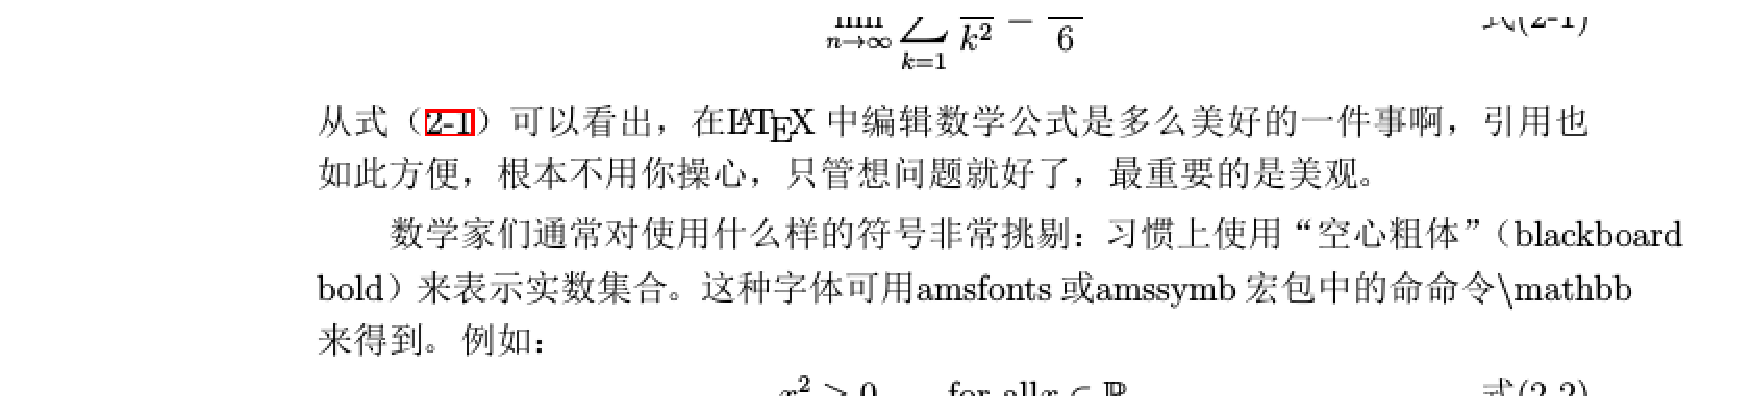
\includegraphics[width=1\textwidth]{overflow}}
 \caption{行溢出}
 \label{fig:amss1}
\end{figure}

这样的话,也是需要你在适当的地方换行。如果你想用他这种,自己写的时候稍微注意一下也可以,你只需要把上面那个变量注释掉就行了。

\section{版权问题}

尊重版权,保证自由,鼓励开源,不建议收费- -

GNU License

\section{问题反馈}

如果模板有问题,你可以自己改改,我也欢迎和我讨论交流:

\href{derektanko@gmail.com}{derektanko@gmail.com}

祝各位顺利毕业,升职加官,当CEO,娶白富美(or嫁高富帅),早得贵子,延续人类,(入土为安)。